%                 _______ ____________  _    _ ______
%                /  ____//  ____/\_   \| \  / ||  ___\
%               /  /___  |  \__   | |\/|  \/  ||  |___
%              /   ___/  \___  \  | |  |      ||   ___\
%             /  /____  ____/  / _| |_ | |\/| ||  |____
%            /_______/ /______/ /_____/|_/  \_||_______\
%        Escuela Superior de Ingeniería Mecánica y Eléctrica 
% ---------------------------------------------------------------
% Erick Vázquez  - IPN ESIME Zacatenco - 15 Septiembre 2015
% ---------------------------------------------------------------
%
% Este es el documento TEX que edite para presentar mi tesis de licenciatura, hago publico este documento ya que a lo largo del desarrollo de mi tesis note que mis compañeros tenían demasiados problemas con el hecho de tener que hacer sus formatos en MS WORD al punto de no poder completar el contenido de sus tesis.

% La intención de compartir este documento es intentar ayudar a aquellos compañeros que tomen el reto de utilizar LaTeX para escribir su trabajo de tesis y puedan enfocarse más en su trabajo de investigación que en la edición de un formato que idealmente nuestra escuela debería proporcionar.

%Este documento tiene el formato de una tesis tradicional con el formato de citas de la IEEE, cada capítulo de esta plantilla viene en un archivo TEX distinto para facilitar la edición y navegación, al inicio de cada sección contiene comentarios para el apoyo de la escritura del contenido del capítulo con el fin de servir como guía para la escritura de la tesis.

%La estructura del documento se editó utilizando la metodología LGS y el libro Como elaborar y asesorar una tesis de Carlos Muñoz Rubio, anexo los documentos en los que se basó el diseño de este formato, pueden ser encontrados en la carpeta Guías en el menú de navegación

% Sientase con la libertad de utilizar, editar y modificar el formato a su gusto    
%
% Se agradece de antemano un agradecimiento a su servidor por la plantilla ;)

%   ergovazquez@esimez.mx            https://github.com/vazeri/
% ---------------------------------------------------------------------------------------------------------
% Inicio del archivo main de configuración

\documentclass[11pt]{report}                  % Tamaño de letra y tipo de documento
\usepackage[spanish]{babel}                   % Indica que escribiremos en español
\usepackage[utf8]{inputenc}     
\usepackage[acronym, toc]{glossaries}         % Agrega glosario
\usepackage{floatrow}
\floatsetup[table]{capposition=top}
\bibliographystyle{unsrt}                     % Orden numérico

\usepackage{titlesec} \linespread{1.25}

\setlength{\parindent}{3em}                   % Separación espacios después del punto y aparte
\setlength{\parskip}{1em}
\setlength{\parindent}{0em}                   % Elimina la sangría francesa

\usepackage{array}
\usepackage{ragged2e}
\usepackage{amssymb}                          % Símbolos matemáticos (por lo tanto)
\usepackage{graphicx} \usepackage{rotating}   % Incluir imágenes en LaTeX
\usepackage{color}                            % Para colorear texto
\usepackage{subfigure}                        % subfiguras
\usepackage{float}                            % Podemos usar el especificador [H] en las figuras para que se queden en su lugar
\usepackage{sidecap}                          % Para poner el texto de las imágenes al lado
\sidecaptionvpos{figure}{c}                   % Para que el texto se alinee al centro 
\usepackage{caption}                          % Para poder quitar numeración de figuras

\usepackage[nottoc]{tocbibind}
\usepackage{anysize} \marginsize{1.5cm}{1cm}{1cm}{1cm} %Margenes Izquierda, derecha, arriba, abajo

\usepackage{titlesec}

\titlespacing\section{0pt}{12pt plus 4pt minus 2pt}{0pt plus 2pt minus 2pt}
\titlespacing\subsection{0pt}{12pt plus 4pt minus 2pt}{0pt plus 2pt minus 2pt}
\titlespacing\subsubsection{0pt}{12pt plus 4pt minus 2pt}{0pt plus 2pt minus 2pt}

\usepackage{titlesec}               %http://ctan.org/pkg/titlesec
\titlespacing{\chapter}{0pt}{30pt}{<after-sep>}% 

\usepackage{appendix}
\renewcommand{\appendixname}{APÉNDICE} \renewcommand{\appendixtocname}{APÉNDICE} \renewcommand{\appendixpagename}{APÉNDICE} 
% Referencias sean hipervínculos a las figuras o ecuaciones y  aparezcan en color
\usepackage[colorlinks=true,citecolor=blue,linkcolor=blue]{hyperref}
\usepackage{fancyhdr} \usepackage{datetime}

\newdateformat{monthyeardate}{\monthname[\THEMONTH], \THEYEAR}
  
\pagestyle{fancy}
\fancyhf{}
\fancyhead[LE,RO]{E.S.I.M.E. Zacatenco}
\fancyhead[RE,LO]{Instituto Politécnico Nacional}
\fancyfoot[CE,CO]{\rightmark}
\fancyfoot[LE,RO]{\thepage}
  
\usepackage{listings}                       % Para usar código fuente
\definecolor{dkgreen}{rgb}{0,0.6,0}         % Definimos colores para usar en el código
\definecolor{gray}{rgb}{0.5,0.5,0.5}        % configuración para el lenguaje a utilizar

\lstset{language=Matlab, keywords={break,case,catch,continue,else,elseif,end,for,function,  global,if,otherwise,persistent,return,switch,try,while}, basicstyle=\ttfamily, keywordstyle=\color{blue}, commentstyle=\color{red}, stringstyle=\color{dkgreen}, numbers=left, numberstyle=\tiny\color{gray}, stepnumber=1, numbersep=10pt, backgroundcolor=\color{white}, tabsize=4, showspaces=false, showstringspaces=false}
   
%\usepackage[backend=biber, style=numeric, citestyle=reading ]{biblatex}  %Restaura citas en pie de pagina 
%\usepackage[backend=biber, style=ieee, citestyle=reading]{biblatex}


\usepackage{biblatex}
\usepackage{footnote} \makesavenoteenv{figure} \makesavenoteenv{tabular} \makesavenoteenv{table}

\addbibresource{Bibliografia.bib}

\thispagestyle{empty}
\usepackage{helvet}                                         % Tipo de letra
\renewcommand{\familydefault}{\sfdefault}

\usepackage{csquotes}

\titleformat{\chapter}[display]                             % No de capitulo
{\normalfont\huge\filleft\bfseries}
{\chaptertitlename \space \thechapter }{0pt}                % Espacio vert despues de capitulo No
{\Huge}[\vspace{1pt}{\titlerule[2pt]}]
\titleformat{name=\chapter,numberless}[display]
{\normalfont\huge\filleft\bfseries}{}{-50pt}                % Títulos de índice
{ \vspace{2ex}\Huge}[\vspace{1ex}{\titlerule[2pt]}]
\titlespacing*{\chapter} {0pt}{-50pt}{20pt}                 % adjust these numbers
\titlespacing*{name=\chapter,numberless} {0pt}{-50pt}{20pt} % adjust these 

\makeglossaries % Es la identificación de todos los conceptos y términos clave que se utilizarán para el desarrollo de la tesis. Lo importante es que el alumno exprese e identifique, con sus propias palabras, las principales definiciones que conoce del tema propuesto y que están relacionadas con su tema. Exprese esos términos como los conoce y los entiende. De esta manera, se podrá evaluar más objetivamente su conocimiento real sobre el tema.

\newglossaryentry{ADC}
{
  name=ADC,
  description={(Convertidor Analógico Digital)  Del inglés "Analog-to-Digital Converter",es un dispositivo electrónico capaz de convertir una señal analógica de tensión en una señal digital con un valor binario}
}

\newglossaryentry{formula}
{
    name=formula,
    description={A mathematical expression}
}

\newglossaryentry{SIBC}
{
  name=SIBC,
  description={(Sistema de Información Basado en Computadoras) Es la integración de hardware, software, personas, procedimientos y datos. Todos estos elementos se conjugan, trabajando juntos, para proporcionar información básica para la toma de decisiones con mayor calidad y facilidad.  }
}

\newglossaryentry{CFE}
{
  name=C.F.E.,
  description={(Comisión Federal de Electricidad)  es una empresa productiva del Estado, encargada de controlar, generar, transmitir y comercializar energía eléctrica en todo el territorio mexicano }
}

\newglossaryentry{CC}
{
  name=C.C.,
  description={ (Corriente Continua)  se refiere al flujo continuo de carga eléctrica a través de un conductor entre dos puntos de distinto potencial, que no cambia de sentido con el tiempo. [ Electrotecnia, ciclos formativos. Peter Bastian]
}
}

\newglossaryentry{CA}
{
  name=C.A.,
  description={ (Corriente Alterna) a la corriente eléctrica en la que la magnitud y el sentido varían cíclicamente. La forma de oscilación de la corriente alterna más comúnmente utilizada es la oscilación senoidal con la que se consigue una transmisión más eficiente de la energía [La corriente alterna, IES, Gerald Brenan.]
}
}

\newglossaryentry{HTML}
{
  name=HTML,
  description={ Lenguaje de marcas de hipertexto (por sus siglas en ingles), es lenguaje para la elaboración de páginas web es un estándar que sirve de referencia para la elaboración de páginas web en sus diferentes versiones, define una estructura básica para la definición de contenido de una página web]
}
}

\newglossaryentry{FP}
{
  name=F.D.P.,
  description={ (Factor De Potencia) Es la relación entre la potencia activa, y la potencia aparente, Da una medida de la capacidad de una carga de absorber potencia activa.[Antonio Gómez Expósito; Fundamentos de teoría de circuitos.]
}
}

\newglossaryentry{FIDE}
{
  name=FIDE,
  description={ (Fideicomiso para el Ahorro de Energía Eléctrica) Fideicomiso privado, sin fines de lucro, constituido el 14 de agosto de 1990, por iniciativa de la Comisión Federal de Electricidad (CFE), en apoyo al Programa de Ahorro de Energía Eléctrica; para coadyuvar en las acciones de ahorro y uso eficiente de la energía eléctrica. 
}
}

\newglossaryentry{PROFECO}
{
  name=PROFECO,
  description={ (Procuraduría Federal del Consumidor) organismo público descentralizado e independiente de la Secretaría de Economía del Gobierno Federal Mexicano. Fue creado para promover y proteger los derechos del consumidor, fomentar el consumo inteligente y procurar la equidad y seguridad jurídica en las relaciones entre proveedores y consumidores
}
}

\newglossaryentry{DAC}
{
  name=D.A.C,
  description={ (Tarifa de alto consumo) Tarifa doméstica de alto consumo, es una multa que cobra la CFE por exceder un límite de consumo en KWh (kilowatt-hora) en su hogar.
}
}

\newglossaryentry{DBMS}
{
  name=DMBS,
  description={ (Sistema de Administración de Bases de Datos) Sistema de administración de bases de datos. Software que controla la organización, almacenamiento, recuperación, seguridad e integridad de los datos en una base de datos}
}

\newglossaryentry{SGBD}
{
  name=SGBD,
  description={ (Sistema de Gestion de Bases de Datos) conjunto de programas que permiten el almacenamiento, modificación y extracción de la información en una base de datos, además de proporcionar herramientas para añadir, borrar, modificar y analizar los datos.}
}

\newglossaryentry{SQL}
{
  name=SQL,
  description={ (Lenguaje de consulta estructurado) por sus siglas en inglés Structured Query Language es un lenguaje declarativo de acceso a bases de datos relacionales que permite especificar diversos tipos de operaciones en ellas.}
}

\newglossaryentry{IP}
{
  name=IP,
  description={ (Dirección IP) Es una etiqueta numérica que identifica, de manera lógica y jerárquica, a una interfaz (elemento de comunicación/conexión) de un dispositivo (habitualmente una computadora) dentro de una red que utilice el protocolo IP (Internet Protocol), que corresponde al nivel de red del modelo OSI}
}

\newglossaryentry{WiFi}
{
  name=WiFi,
  description={ Mecanismo de conexión de dispositivos electrónicos de forma inalámbrica.}
}

\newglossaryentry{PCB}
{
  name=PCB,
  description={ (Placa de Circuito Impreso) Superficie constituida por, pistas o buses de material conductor laminadas sobre una base no conductora. El circuito impreso se utiliza para conectar eléctricamente a través de las pistas conductoras.}
}

\newglossaryentry{TVS}
{
  name=TVS,
  description={ (Supresores para transitorios de voltaje) Diodo usado para proteger componentes electrónicos de descargas electrostáticas causadas por picos de voltaje inducidos en cables o pistas de circuitos [ What are TVS diodes, Semtech Application Note SI96-01] }
}

\newglossaryentry{NOM}
{
  name=NOM,
  description={ (Normatividad Mexicana) Serie de normas cuyo objetivo es regular y asegurar valores, cantidades y características mínimas o máximas en el diseño, producción o servicio de los bienes de consumo entre personas morales y/o personas físicas, sobre todo los de uso extenso y de fácil adquisición por parte del público en general [Asociación de Normalización y Certificación, 2015] }
}

\newglossaryentry{IEEE}
{
  name=IEEE,
  description={ (Instituto de Ingeniería Eléctrica y Electrónica) Asociación mundial de técnicos e ingenieros dedicada a la estandarización y el desarrollo en áreas técnicas. [ IEEE at a Glance 2011] }
}

\newglossaryentry{ESD}
{
  name=ESD,
  description={ (Descarga electrostática) es un fenómeno electrostático que hace que circule una corriente eléctrica repentina y momentáneamente entre dos objetos de distinto potencial eléctrico; como la que circula por un pararrayos tras ser alcanzado por un rayo se utiliza para describir las corrientes indeseadas momentáneas que pueden causar daño al equipo electrónico. [Fundamentals of Electrostatic Discharge, An Introduction to ESD, 2013, ESD Association] }
}

\newglossaryentry{AVR}
{
  name=AVR,
  description={ Familia de microcontroladores RISC del fabricante estadounidense Atmel. El acrónimo AVR no significa nada en particular deacuerdo a ATMEL  [Embedded C Programming and the Atmel AVR, Larry O'Cull, 2006] }
}

\newglossaryentry{LGS}
{
  name=LGS,
  description={ Metodología de desarrollo de sistemas de información basados en computadora  [Herrera Martínez Alejandro ] }
}

\newglossaryentry{AWG}
{
  name=AWG,
  description={ (Calibre de alambre estadounidense) Referencia de clasificación de diámetros para conductores eléctricos (cables) indicados con la referencia AWG. Cuanto más alto es este número, más delgado es el alambre. El alambre de mayor grosor (AWG más bajo) es menos susceptible a la interferencia, posee menos resistencia interna y, por lo tanto, soporta mayores corrientes a distancias más grandes.  [Servicios Condumex (2005) Manual técnico de cables de energía ] }
}


\newglossaryentry{RMS}
{
  name=RMS,
  description={ (Valor Cuadrático Medio) Denominado valor eficaz. Se define como el valor de una corriente rigurosamente constante (corriente continua) que al circular por una determinada resistencia óhmica pura produce los mismos efectos caloríficos (igual potencia disipada) que dicha corriente variable (corriente alterna)  [Fundamentos de Circuitos Eléctricos, Charles K. Alexander, 2012] }
}


\newglossaryentry{CFL}
{
  name=CFL,
  description={ (Lámpara Fluorescente Compacta)  es un tipo de lámpara que aprovecha la tecnología de los tradicionales tubos fluorescentes para hacer lámparas de menor tamaño que puedan sustituir a las lámparas incandescentes con pocos cambios en la armadura de instalación y con menor consumo   }
}

\newglossaryentry{UART}
{
      name=UART,
  description={ (Transmisor-Receptor Asíncrono Universal) es el dispositivo que controla los puertos y dispositivos serie. Se encuentra integrado en la placa base o en la tarjeta adaptadora del dispositivo.  [Alternativas al bajo consumo CFL] }
}


\newglossaryentry{ENIG}
{
      name=ENIG,
  description={ (Electrolítico de oro de inmersión de níquel) Tipo de recubrimiento utilizado para placas de circuito impreso. Se compone de un recubrimiento de níquel no electrolítico cubierto con una fina capa de oro de la inmersión, que protege el níquel de la oxidación. [ "Surface Finishes in a Lead Free World, Uyemora International 2014] }
}
\newglossaryentry{IDE}
{
      name=IDE,
  description={(Integrated Development Environment) Es un ambiente de desarrollo interactivo o entorno de desarrollo integrado  es una aplicación de software, que proporciona servicios integrales para facilitarle al programador de computadora el desarrollo de software }
}

\newglossaryentry{TDH}
{
      name=TDH,
  description={ (Distorsión armónica total) Es la relación entre el contenido armónico de la señal y la primera armónica o fundamental. La distorsión armónica total nunca debe estar por encima del 1\%. De estarlo, en lugar de enriquecer la señal, la distorsión empieza a desvirtuarla }
}

\newglossaryentry{KWh}
{
      name=KWh,
  description={ (Killowatt Hora) Es una unidad de energía equivalente a 1000 watts por hora o 3.6 mega joules si la energía es transmitida o usa a un ritmo constante  (potencia) sobre un periodo de tiempo la energía total es el producto de la potencia por el tiempo , usualmente se utiliza como unidad de cobro para la energía consumida por usuarios de instalaciones eléctricas ["Thompson, Ambler and Taylor, Barry N. (2008). Guide for the Use of the International System of Units (SI) "] }
}

\newglossaryentry{watt}
{
      name=watt,
  description={  El vatio o watt es la unidad de potencia del Sistema Internacional de Unidades. Su símbolo es W. Expresado en unidades utilizadas en electricidad, un vatio es la potencia eléctrica producida por una diferencia de potencial de 1 voltio y una corriente eléctrica de 1 amperio (1 voltiamperio). ["Diccionario de la lengua española (22.ª edición), Real Academia Española, 2001, consultado el 21 de marzo de 2015."] }
}

\newglossaryentry{LED}
{
      name=LED,
  description={ (Light-Emitting Diode) ‘diodo emisor de luz’; es un componente optoelectrónico pasivo y, más concretamente, un diodo que emite luz.}
}

\newglossaryentry{VAR}
{
      name=VAR,
  description={ (Volt Amper Reactivo) Potencia que no posee un carácter realmente de ser consumida; sólo aparece cuando hay bobinas o condensadores en los circuitos. Dicha potencia tiene un valor medio nulo, por lo que no produce trabajo necesario. 
  }
  }


\newglossaryentry{MOS}
{
      name=MOS,
  description={ MOS Technology, Inc., también conocida como $Commodore Semiconductor Group$, (al ser adquirida por CBM), fue un fabricante de calculadoras y microprocesadores, siendo famosa por su microprocesador MOS Technology 6502. [Información sobre los chips MOS y su uso en los ordenadores – Ronald van Dijk]
}
}

\newglossaryentry{USB}
{
      name=USB,
  description={ ( Universal Serial Bus) El Bus Universal en Serie (BUS), más conocido por la sigla USB, es un bus estándar industrial que define los cables, conectores y protocolos usados en un bus para conectar, comunicar y proveer de alimentación eléctrica entre computadoras, periféricos y dispositivos electrónicos. [Boston Globe Online  USB deserves more support. Simson.net. 31 de diciembre de 1995]
  }
  }

\newglossaryentry{FTDI}
{
      name=FTDI,
  description={ (Future Technology Devices International), comúnmente conocida por su abreviatura FTDI, es una empresa privada escocesa de dispositivos semiconductores, especializada en tecnología Universal Serial Bus. }
}
 \renewcommand*{\glstextformat}[1]{\textbf{#1}}


\begin{document}

%%%                                 INICIA 
\begin{center}																		%%%
\newcommand{\HRule}{\rule{\linewidth}{0.6mm}}									%%%\left
 																					%%%
\begin{minipage}{0.48\textwidth} \begin{flushleft}

\includegraphics[scale = 0.25]{Tesis/Imagenes/IPN}
\end{flushleft}\end{minipage}
\begin{minipage}{0.48\textwidth} \begin{flushright}

\includegraphics[scale = 0.23]{Tesis/Imagenes/Esime_Logo_Modificado.png}
\end{flushright}\end{minipage}

\pagestyle{empty} % No headers
													 								%%%
\vspace*{-1.5cm}								%%%
																					%%%	
\textsc{\LARGE  INSTITUTO POLITÉCNICO NACIONAL}\\[1.5cm]	

\textsc{\LARGE Escuela Superior de Ingenier\'ia\\ Mecánica y Eléctrica\\ \vspace{8px} \Large Unidad Profesional Zacatenco}\\[.15cm]				

\vspace{8px} \small  INGENIERÍA EN COMUNICACIONES Y ELECTRÓNICA \\[1.5cm]				
%%%

\begin{minipage}{0.9\textwidth} 

\begin{center}																					%%%
\textsc{\huge TRABAJO TERMINAL } % Se convierte en tesis de acuerdo a la evaluación de los sinodales en el examen profesional

%El  Trabajo de Grado debe tener un componente investigativo, que consiste en la formulación, planeación y en algunos casos, ejecución de un trabajo o proyecto en el que el estudiante ponga en práctica los conocimientos adquiridos en el transcurso del programa académico.
 
%De esta manera, el trabajo de grado se convierte en una oportunidad para la fundamentación, aplicación y producción de conocimientos, que conjuguen las habilidades investigativas con los saberes y competencias adquiridas a través de la formación académica y profesional, y a partir de los cuales se planteen soluciones a los problemas de su contexto social y laboral.

\end{center}

\end{minipage}\\[0.5cm]
%%%
    																				%%%
 			\vspace*{1cm}																		%%%
																					%%%
{ \huge \bfseries Guía, esquema, cuerpo del escrito 
para trabajo de grado de licenciatura\\[0.03cm] } 

% La elección del tema de tesis debe ser congruente con la carrera que se cursa, (con el mapa curricular o área de estudio) Sera evalúa por un jurado, debe buscar la solución de una problemática real, y debe ser pertinente con los estándares de la escuela )

% La tesis de licenciatura debe cubrir la suma de técnicas o modificación de una, es una propuesta de soluciones a una problematica real.

% El titulo tentativo del trabajo, esta en constante cambio conforme al desarrollo del trabajo, no te enamores de un solo titulo ni te preocupes tanto por que sea el adecuado, ya que al final del trabajo, los asesores que te hagan tus revisiones, terminan modificandolo. 	

\vspace*{1.5cm}%%%
							%%%
 								%%%
\begin{minipage}{0.46\textwidth}													%%%
\begin{flushleft} \large															%%%
P R E S E N T A N:\\	

\vspace*{.4cm}%%%

Autor 1\\     % Se permiten de 1 a 3 compañeros en un solo equipo para el desarrollo de la tesis 
Autor 2\\
Autor 3\\
\space
%%%
			%
            \vspace*{1.2cm}	
            													%%%
										 						%%%
\end{flushleft}																		%%%
\end{minipage}		
																%%%
\begin{minipage}{0.52\textwidth}		
\vspace{-0.6cm}											%%%
\begin{flushright} \large															%%%
A S E S O R E S: \\		
\vspace*{.4cm}%%%

Asesor Metodológico\\    % El asesor metodológico es el profesor asignado en la materia de DPP, (No se puede cambiar)
Asesor Técnico 1\\       % Los asesores técnicos, pueden ser elegidos por los autores de la tesis de la especialidad 
Asesor Técnico 2\\       % o de una especialidad ajena en a la que se esta cursando (Tu los elijes)

% Es importante destacar que los asesores ganan puntos por cada trabajo de grado que pasa como tesis, entre mas puntos acumulan tienen acceso a mejores prestaciones económicas por parte de la escuela, existen profesores caza puntos, que lo único que buscan es ser anotados como asesores y se esconden o simplemente no ayudan a los alumnos en sus trabajos de tesis, así que debes asegurarte de que tus asesores sean personas integras, con conocimientos que puedan ayudarte en el desarrollo de tu tesis. 

% El trabajo del asesor metodológico es darte a entender cual es el formato del trabajo, el propósito y forma de la tesis, apoyarte con tus exposiciones, y procurar que este bien redactado. Usualmente no se meten en la parte técnica.

% El trabajo de los asesores técnicos es procurar verificar que lo que estés haciendo técnicamente, a ellos se les suele entregar una copia de tus avances del escrito para que la revisen y te hagan anotaciones, correcciones de gramática y ortografía, así como también es parte de su labor apoyarte y buscar la manera de defender tu tesis ante los profesores que serán los sinodales que te evaluaran en la defensa de tu examen profesional 

\end{flushright}																	%%%
\end{minipage}	
\vspace*{1cm}

\begin{center}	

\textsc{\LARGE para obtener el titulo de:}\\[.5cm]		

 		\large{\textbf{\Large Ingeniero en comunicaciones y electrónica}	}\ % Cambiar si corresponde														%%%
\vspace{.5cm} 																				
																				
{\large México, D.F. \monthyeardate \today }	%Actualiza la fecha automáticamente, el día no debe ir en la portada solo el mes y año												%%%
 			\end{center}\end{center}		
 			 			\vspace{.1cm} 	
																		
%%%%%%%%%%%%%%%%%%%% TERMINA PORTADA %%%%%%%%%%%%%%%%%%%%%%%%%%%%%%%%
%%%%%%%%%%%%%%%%%%%%%%%%%%%%%%%%%%%%%%%%%%%%%%%%%%%%%%%%%%%%%%%%%%%%%%%%%%%%%%%%%%%%%
% Protocolo de la tesis
%%%%%%%%%%%%%%%%%%%%%%%%%%%%%%%%%%%%%%%%%%%%%%%%%%%%%%%%%%%%%%%%%%%%%%%%%%%%%%%%%%%%%

% El protocolo es la parte mas importante para los asesores, ya que con esta es posible que entiendan la totalidad del trabajo en un par de paginas, si necesidad de leer todo el trabajo, en caso de querer ahondar mas en el trabajo se dirigirán al índice en donde solo con revisarlo deberán entender a grandes rasgos el como se desarrollo el trabajo de tesis 

\newpage %Termina la pagina actual y desplaza el contenido a una nueva pagina
\newpage


\newpage
~\vfill
%\thispagestyle{empty}

\emph{DEDICATORIA}
\hfill \break

La dedicatoria es un breve texto, que se escribe al principio  o al final de un libro, tesis, película, canción, etc., para expresar agradecimiento por el apoyo o ayuda en el desarrollo y finalización de la obra, sea del género  o formato que fuere esta. Dirigidas hacia una persona, personas o instituciones  a las que se agradece por su ayuda o apoyo.   

La palabra tesis significa "proposición o conclusión que se mantiene por razonamiento”. Se entiende por tesis a la  disertación escrita que se presenta para la obtención de un título, licenciatura, doctorado, o como conclusión de un estudio especializado de un tema en particular. Por lo común la tesis se presenta al terminar los estudios, pero se puede empezar  a escribir en cualquier momento de los mismos.

Esto deja entender que una dedicatoria de tesis, está dirigida a aquellos que de alguna forma han sido de ayuda o apoyo para quien la escribe, por cualquier clase de apoyo moral, material, económico o didáctico, proporcionados. Ya sean familiares, amigos, profesores o compañeros, y  aquellos que hayan intervenido de alguna forma en el desarrollo de las ideas y experiencias que tengan como conclusión la culminación de la tesis en cuestión y a los que el autor de la misma pretenda agradecer por medio de la dedicatoria, como en el caso de maestros, compañeros, asesores, e impresores, que  de alguna forma contribuyeron a la culminación de la tesis, así como a los sinodales por aprobarla, quienes califican si en la tesis se cumplieron los objetivos de la misma, como, cuál es el problema planteado en la tesis y cuál  la propuesta de solución al problema,  qué estuvo mal en la metodología y si fueron corregidos o rectificados por la tesis en cuestión.

Generalmente las dedicatorias son breves, no más de dos o tres líneas, aunque también hay dedicatorias muy largas \cite{Dedicatoria}.

\text
\hfill \break

\noindent \textsc{Vázquez González Erick}\\

\noindent \textsc{ergovazquez@esimez.mx}\\ % URL

\noindent \textsc{Escuela Superior de Ingeniería Mecánica y Eléctrica, Unidad Zacatenco}\\

\noindent Ultima Revisión \today{} % Printing/edition 

\newpage
\thispagestyle{empty}

\section*{Introducción} % El * omite la sección del índice 

\textit{Una breve introducción que explique el por que se esta desarrollando el trabajo Así como, empezar a definir, el Producto Principal del Proyecto  de Tesis y empezar a concebir el Objetivo o Alcance Principal del Proyecto, lo cual, como se comentó antes, “es mejorar la calidad del medio ambiente”} \cite{Tesis}.


\section*{Antecedentes}

\textit{Aquí el alumno tiene que manifestar, en palabras cotidianas, todo lo que conoce sobre el tema que pretende desarrollar, de la manera más amplia y completa posible. Es deseable que indique sus referencias sobre el tema, las teorías, los conceptos y los conocimientos implicados en éste, así como la bibliografía y todos los posibles detalles que permitirán evaluar la profundidad de su conocimiento sobre el tema. Es indispensable tomar en cuenta el estado del arte de la temática propuesta.}

\textit{El objetivo de esta sección del proyecto es conocer qué tanto sabe y entiende del tema el alumno, para contar con elementos de juicio sobre sus posibilidades de desarrollo de la investigación propuesta.}

\section*{Alcances}

\textit{En este apartado del proyecto el alumno debe establecer hasta dónde llegará con su estudio, qué tanto pretende abarcar y qué dejará sin examinar en su investigación. Se trata de que el propio alumno delimite las fronteras de su trabajo, de manera que no rebase lo esperado, pero tampoco se quede por debajo de los límites establecidos.}

\textit{Es necesario señalar que no todos los temas propuestos son factibles de investigar, ya sea teórica o empíricamente; por eso hay que establecer los límites dentro de los cuales se puede actuar.}

\section*{Justificación}

\textit{Expresar, en palabras sencillas y de manera breve, las razones por las cuales desea investigar ese tema de tesis, ya sea personales, académicas, profesionales o de otra índole. }

\textit{Para el asesor es quizá el elemento más importante de la propuesta, ya que le permitirá evaluar la posibilidad de que el alumno lleve a término su investigación, en tanto que podrá valorar sus limitaciones, alcances, disponibilidad y conocimientos, entre otros muchos aspectos.}

\newpage

\section*{Objetivos}

\textit{Este apartado expresa, en palabras llanas y simples, cuál será el fin último que se pretende alcanzar con la tesis. El objetivo se determina respondiendo a estas interrogantes: ¿qué se quiere hacer?, ¿qué se pretende alcanzar?, ¿cómo se puede analizar? y ¿qué se quiere demostrar?}

\subsection*{Objetivo general}

\textit{Inherentes con un Sistema, que se desarrollará como parte del Proyecto completo.}

Generar un sistema de monitoreo eléctrico con la capacidad de medir la potencia real de una instalación eléctrica con precisión.

\subsection*{Objetivos específicos}

\textit{La suma de los objetivos específicos debe dar el objetivo global o general.}

\begin{itemize}

	\item Conocer el medio y métodos de medición del consumo eléctrico.
	\item Diseñar un sistema que permita medir y procesar la potencia real de una instalación monofásica.
	\item Construir un \gls{SIBC} para almacenar dichos parámetros. 
	\item Medir la corriente de la instalación con un bajo margen de error con forme a la norma Norma Oficial Mexicana 001-SEDE-2012. 

\end{itemize}
  

\section*{Resumen} 

\textit{Se presenta un pequeño resumen que permita al lector recopilar toda la información del protocolo para así poder proceder al primer capitulo de la tesis. }

\section*{Resume} %Se recomienda presentar el resumen en ingles

\textit{Es una copia en ingles de la sección anterior con el propósito de permitir que lectores de otros países encuentren el documento.}

\newpage  

\setlength{\parindent}{0em}                   % Separación espacios después del punto y aparte
\setlength{\parskip}{0em}                     % ÍNDICE COMPACTO
\tableofcontents                              % Índice general
\listoftables                                 % Índice de tablas 
\listoffigures                                % Índice de figuras

\clearpage \printglossary   \printglossary[type=\acronymtype]

\setlength{\parskip}{.3cm}                    % PUNTOS Y APARTE párrafos
\setlength{\parindent}{0cm}                   % Sangría francesa
\setlength{\abovecaptionskip}{-20pt}          % espacio antes de figuras y tablas
\setlength{\belowcaptionskip}{-20pt}          % espacio después de figuras y tablas
\setlength{\abovedisplayshortskip}{-10pt}     % Espacio después de ecuaciones
\setlength{\belowdisplayshortskip}{10pt}      % Espacio ante/después de ecuaciones
\addtolength{\parskip}{-0.75mm}

\let\OLDitemize\itemize
\renewcommand\itemize{\OLDitemize\addtolength{\itemsep}{-10pt}}     % Espacio entre viñetas

% Capítulo I Marco Conceptual

% El marco conceptual o marco teórico, presenta de manera breve y concisa la teoría involucrada en el proyecto, es importante mantener un orden en la estructura del documento es indispensable manejar Capítulos, secciones y sub-secciones, estos comandos generan automáticamente el índice general que servirá a los asesores para navegar el documento. 

\chapter{ MARCO CONCEPTUAL }

\textit{El marco conceptual contiene de manera breve toda la teoría necesaria para poder entender el contenido de los siguientes capítulos.}

\section{ Ley de Ohm }

\begin{figure}[H]
	\begin{center}
 		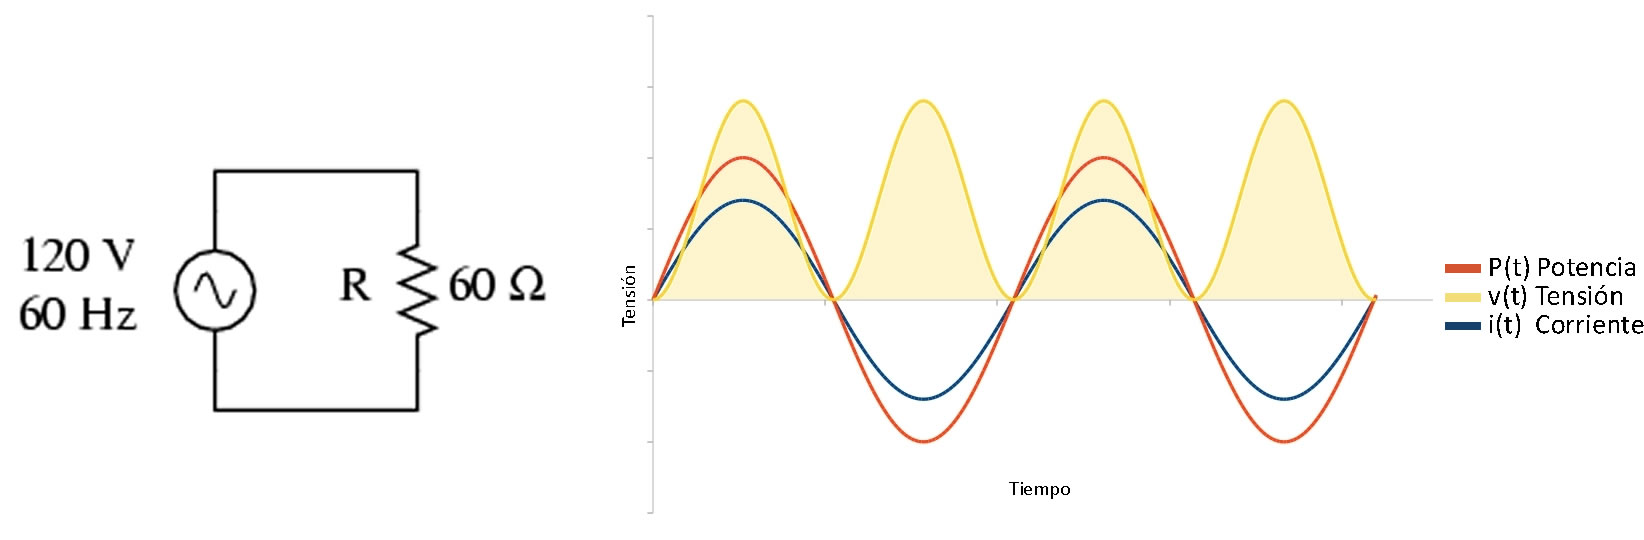
\includegraphics[width = .8\textwidth]{Tesis/Imagenes/resistiva.jpg}
 		\captionof{figure}{Comportamiento en el tiempo de una carga resistiva \cite{AC}} 
	\label{RESISTIVA}
    \end{center} 
\end{figure}

Es una de las leyes fundamentales de la electrodinámica, estrechamente vinculada a los valores de las unidades básicas presentes en cualquier circuito eléctrico como son:

\begin{equation}
V = IR  
\label{voltaje}
\end{equation}

A las formula de en la ecuación \ref{voltaje} se le conoce como la Ley de Ohm

\subsection{ Despeje de la ley de ohm }

Es posible despejar la corriente de la ecuación \ref{voltaje} para poder obtener la corriente total que fluye por el sistema dando como resultado la ecuación \ref{corriente} es decir:

\begin{equation}
I = V/R  
\label{corriente}
\end{equation}

\begin{itemize}
\item Tensión o voltaje $E$, en volt ($V$).
\item Intensidad de la corriente $I$, en ampere ($A$).
\item Resistencia $R$ en ohm ( $\Omega$ ) de la carga o consumidor conectado al circuito.
\end{itemize}

\section{ Resumen del capitulo 1 }

\textit{Para ayudar al lector se recomienda agregar una sección de resumen del capitulo, esto permite al lector resumir y entender que es los que leyó y dar un repaso del contenido del capitulo así como guiarlo con una referencia de entrada al capitulo siguiente.}


% FIN de Capítulo I Marco Conceptual


% Capítulo II Marco Contextual

%El marco contextual contiene el contexto en el que se esta llevando acabo la tesis (el país, dispositivos similares al que se desarrolla, tipos de sistemas involucrados, normatividades gubernamentales) esto para tener un marco de referencia sobre el cual trabajar los siguientes capítulos.

\chapter{ MARCO CONTEXTUAL }

\textit{El marco contextual es el medio ambiente en donde se desarrolla o desarrollará el proyecto de tesis; el Medio Ambiente Temporal o Histórico; que incluye, sus antecedentes históricos o de creación, y el Medio Ambiente Espacial o Físico, que incluye, la ubicación física de la empresa o área.}

\textit{ Todo esto, sirve para ubicar al lector (y al mismo alumno), en los antecedentes del: Marco Contextual del Medio Ambiente (empresa, área, institución), en donde se desarrollará el proyecto de tesis.}


\section{ Sistemas de monitoreo de energía }

El avance de la tecnología hace que cada vez se desarrollen nuevos sistemas que monitorizan el consumo energético, sin embargo ninguno de ellos cumple con las características necesarias para ser implementados en México esto debido al sistema de cobro implementado en el país. 

\section{ Medición y cobro de la energía en México }

A la fecha, existen en México 43 tarifas distintas para el suministro y venta de energía eléctrica clasificadas de acuerdo con su uso y su nivel de tensión. El esquema tarifario eléctrico que controla la Secretaría de Hacienda, ha privilegiado los subsidios cruzados \footnote{Este es un ejemplo de pie de pagina se utiliza para clarificar las dudas que puedan surgir en el lector a lo largo de la lectura } 

\subsection{ Cables al interior de la instalación eléctrica }

Los calibres dependen de la carga a alimentar, el calibre mínimo a utilizarse es No. 12 \gls{AWG}. Para alimentación exclusiva de lámparas puede utilizarse calibre No. 14 \gls{AWG}. Si es un solo circuito y existe una carga mayor a 3,500 Watts utilizar preferentemente calibre No. 10 para alimentadores principales. Diámetro de la tubería mínimo de 3/4 de acuerdo con la normatividad de la \gls{CFE}

\begin{table}[H]
\centering
\begin{tabular}{||c c c c c||} 
 \hline
 \multicolumn{5}{|c|}{Amperaje que soportan los cables de cobre} \\
 \hline
 mm$^2$  & AWG & Amperaje 60c& Amperaje 75c & Amperaje 90c \\ [0.5ex] 
 \hline\hline
 2.08 & 14 & 15 A& 15 A & 15 A  \\ 
 3.31 & 12 & 20 A & 20 A & 20 A \\
 5.26 & 10 & 30 A& 30 A & 30 A \\
 8.37 & 8 & 40 A& 50 A & 55 A \\
 \hline
\end{tabular}

\caption{Calibres estándar para instalaciones domesticas de acuerdo a su temperatura máxima }
\label{table:cablibres}
\end{table}

\section{ Resumen del capitulo 2 }

Resumen del capitulo e introducción al siguiente capitulo. 
\chapter{ ANÁLISIS, EVALUACIÓN Y DIAGNOSTICO }

\textit{Este capitulo permite establecer un diagnostico general de los sistemas existentes, sobre los cuales se desarrollara el tema de tesis pretende abarcar.}

\section{ Análisis de la situación actual }

\begin{itemize}
	\item  El usuario no entiende de manera clara cuanto es lo que deberá pagar en moneda nacional.

    \item La compañía cambia anualmente los precios de sus tarifas por \gls{KWh}.
    
    \item Dependiendo del consumo existirá o no un subsidio en el recibo por parte del gobierno.
    
\end{itemize}

\section{ Evaluación }

    \textit{Es necesario conocer los dispositivos o sistemas similares al que se pretende desarrollar en este ejemplo se analizan el medidor analógico y el digital}

\subsection{ Medidor analógico mecánico }
    
\subsection{ Medidor inteligente digital }

\section{ Ventajas y desventajas de los sistemas actuales }
    
    La siguiente tabla contiene los sistemas de medición, que se utilizan actualmente para el cobro de la energía eléctrica en México.
    
    \begin{table}[H]
    \centering
    \begin{tabular}{| m{3.8cm} | m{7.3cm}| m{6.2cm} |} 
    \hline
    
    Tipo de Medidor & Ventajas & Desventajas\\
    \hline\hline
    Medidor Digital & Auto protegidos, sensibles a alteraciones, desconexiones, medición digital, Comunicación vía linea  eléctrica hacia la compañía & No ofrece por si mismo Información relevante al usuario , costo elevado para la compañía, desconexión remota de energía. \\
    \hline
    Medidor Analógico (Descontinuado)& Medición por medio de inductores, Mecanismo Mecánico & Fácilmente alterables, ya no están en producción ni distribución\\
    \hline
    \end{tabular}
     \caption{Tabla con los sistemas actuales de medición de energía domestica en México}
     \label{tblsistemas}
    \end{table}

\section{ Diagnostico }

\textit{Utilizando el análisis, ahora es posible establecer un diagnostico de la problemática que se pretende resolver con base en el análisis realizado de los sistemas existentes.}

\section{ Resumen del capitulo 3 }

\textit{Resumen del capitulo e introducción al siguiente capitulo.}
% Capítulo III Marco Metodológico

% Este capitulo cubre la descripción de la metodología, técnicas y herramientas con las cuales se resolverá el o los problemas de esta TESIS (¿con que se va a hacer?)

\chapter{ MARCO METODOLÓGICO }

\section{ Metodología del Sistema de Información  }

\textit{En este punto deben indicarse los métodos, las técnicas y herramientas, que se utilizarán para llevar a cabo la investigación.}

\section{ Hardware }

\textit{En caso de utilizar componentes electrónicos físicos deben describirse de manera breve y concisa.}

\subsection{ Sensor de corriente }

El transformador sensor de corriente Yhdc es fabricado en Beijing YaoHuadechang por Electronic Co., Ltd el modeo, SCT-013-000, con numero de parte SKU THM105C4B. Sera utilizado debido a su capacidad de sensar hasta 100Amperes, cubriendo así los requisitos mínimos de la NOM001 y previendo la instalación del dispositivo en sistemas de mayor consumo de corriente.

\section{ Lenguajes de programación e Internet }

\textit{Para el caso de los lenguajes de programación de igual manera que el hardware se mencionan solo los aspectos mas relevantes de manera breve y concisa. }

\subsection { Hyper Text Markup Language (HTML) }

\textit{Descripción breve de HTML utilizando el sistema de citas (todo lo que se copie y pegue debe estar citado) de otra manera se le considera plagio.}

Lenguaje de marcas de hipertexto, lenguaje utilizado para la elaboración de páginas web es un estándar que sirve de referencia para la elaboración de páginas web en sus diferentes versiones a través de etiquetas, define una estructura básica y un código para la definición de contenido de una página web. Es un estándar a cargo de la $W3C$, organización dedicada a la estandarización de tecnologías ligadas a la web. \cite{html}.

\section{ Resumen del Capitulo 4 }

\textit{Resumen del capitulo e introducción al siguiente capitulo.}

% Capítulo III Marco Metodológico
%Capítulo IV Caso Práctico/Construcción

%; Normalmente el cuerpo principal del Proyecto y documento de la tesis.  Supongamos que; se define qué: el Producto Principal a desarrollar es: Un Sistema de Información Basado en Computadoras [1], y se elige la Metodología de Leopoldo Galindo Soria (LGS), ya qué es la más cercana o la más conocida en ese medio ambiente.  A partir de ahí, se siguen las actividades que sugiere ésta Metodología, para  crear o proponer o construir el Producto Principal del Proyecto de Tesis.

\chapter{ DISEÑO DEL SISTEMA }

\textit{En este capitulo se cubre la implementación del sistema en su conjunto así como los pasos a seguir a grandes rázgos sin entrar en muchos detalles sobre como se diseña el sistema a implementar }

\section{ Requisitos funcionales del sistema }

\begin{itemize}

\item \textbf{Comunicación Inalámbrica:} Debe tener la capacidad de transmitir de manera inalámbrica la medición tomada por el micro controlador

\item \textbf{Restricción de sustancias peligrosas:} La tarjeta debe cumplir con las normas ambientales internacionales (RoHS\footnote{RoHS (De las siglas en inglés Restriction of Hazardous Substances) se refiere a la directiva 2002/95/CE de Restricción de ciertas Sustancias Peligrosas en aparatos eléctricos y electrónicos, adoptada en febrero de 2003 por la Unión Europea}) y evitar el uso de sustancias toxicas en sus materiales y fabricación.
 
\item \textbf{Capacidad de múltiples lecturas:} Se requiere una tarjeta que tenga la capacidad de medir de al menos una fase del sistema eléctrico.

\item \textbf{Lectura del consumo energético:} El usuario podrá colocar un sensor de corriente de manera segura que permita medir la intensidad que circula por el conductor.

\item \textbf{Creación de una cuenta web:} El usuario podrá crear una cuenta en la plataforma web del producto.

\end{itemize}

\section*{ Nivel usuario }

\begin{itemize}

\item Medir el consumo de la instalación eléctrica.
\item Procesar la información.
\item Interpretar la información por medio software en un navegador web.
\item Mostrar la información al usuario de una manera agradable e intuitiva.
\end{itemize}

\section*{ Nivel técnico }

\begin{itemize} 

\item Medir la corriente que fluye por el sistema eléctrico.
\item Procesar la señal por medio de un micro controlador.
\item Elegir un medio de trasmisión para la información.
\item Enviar la información a un servidor web.
\item Simplificar la información de manera gráfica y clara para el usuario.

\end{itemize}


\section*{Nivel sistema}

\begin{itemize} % [noitemsep] removes whitespace between the items for a compact look

\item Acondicionar las señales para el Convertidor Analógico Digital del microcontrolador.
\item Aplicar un corrimiento de \gls{CC} para que el micro controlador pueda leer $2^8$ valores (256).
\item Canalizar por un puerto del micro controlador la señal digitalizada.
\item Enviar la señal de manera inalámbrica a través de un sistema de radio frecuencia.
\item Procesamiento de los datos de entrada del lado servidor.
\item Visualización de los datos a través de una aplicación web.
\end{itemize}


%Capítulo IV Caso Práctico/Construcción


%CAPITULO VI , Análisis de resultados

%Una cosa es lo que se propuso resolver y otra lo que realmente se obtuvo, en esta etapa se analizan los resultados obtenidos como parte del desarrollo del trabajo de investigación. 

\chapter{ ANÁLISIS DE RESULTADOS }

\textit{Es necesario reportar de manera final cual es prototipo y los resultados que se obtuvieron, esto con el fin de generar las conclusiones utilizando los resultados del prototipo generado.}

\section{ Prueba No. 1 - Sistema eléctrico de 4 fases (Calibración)}

La figura \ref{Graficas} contiene la medición de 3 fases utilizando el sistema de medición conectado para realizar una medición no invasiva en un sistema lineal, con una carga netamente resistiva

\subsection{ Objetivo de la prueba}

Verificar el adecuado funcionamiento del dispositivo electrónico, calibrar el software contra dispositivos certificados de nombre reconocido para obtener una medición lo mas exacta posible, con la finalidad de realizar mediciones con la mayor certidumbre posible \cite{NOM}.

\subsection{ Procedimiento}

En el neutro el sensor de corriente correspondiente al puerto CT1 del circuito implementado, por ley de nodos, al ser la carga bajo medición un circuito en con una resistencia en serie, la corriente que fluye por toda la maya debe ser igual en la fase y el neutro, por lo que se procede a realizar la medición.

\begin{figure}[H]
	\begin{center}
 		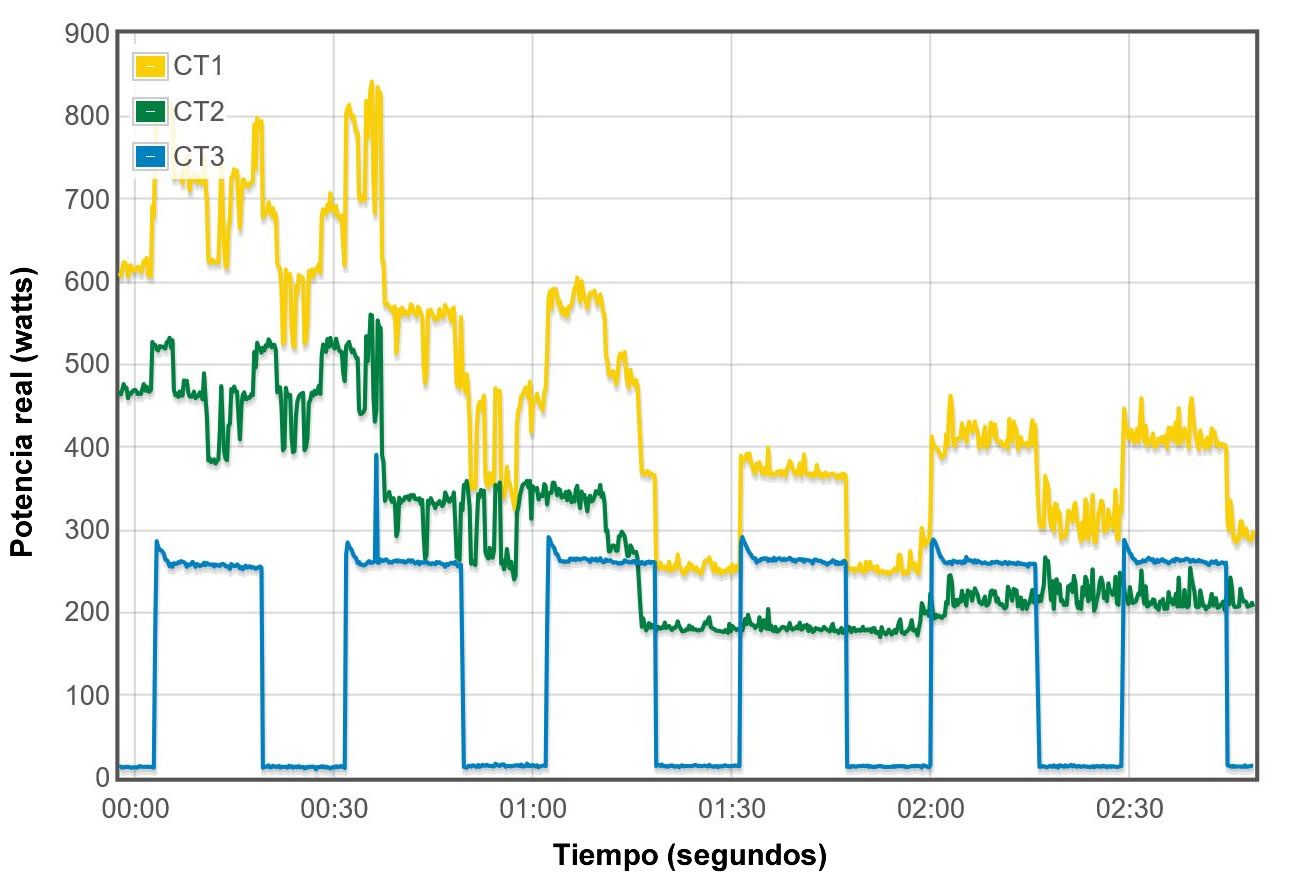
\includegraphics[width = .85\textwidth]{Tesis/Imagenes/Grafica.JPG}
 		\captionof{figure}{Gráfica en tiempo del sistema de medición} 
	\label{Graficas}
    \end{center} 
\end{figure}




%Capitulo V Conclusión/Valoración de objetivos


%Para terminar es necesario revisar los objetivos planteados, verificar su cumplimiento y en caso de no haberse cumplido justificar el por que no se pudo cumplir el objetivo.


\chapter{ CONCLUSIÓNES }

\section{Características finales de la tarjeta}

\begin{figure}[H]
	\begin{center}
 		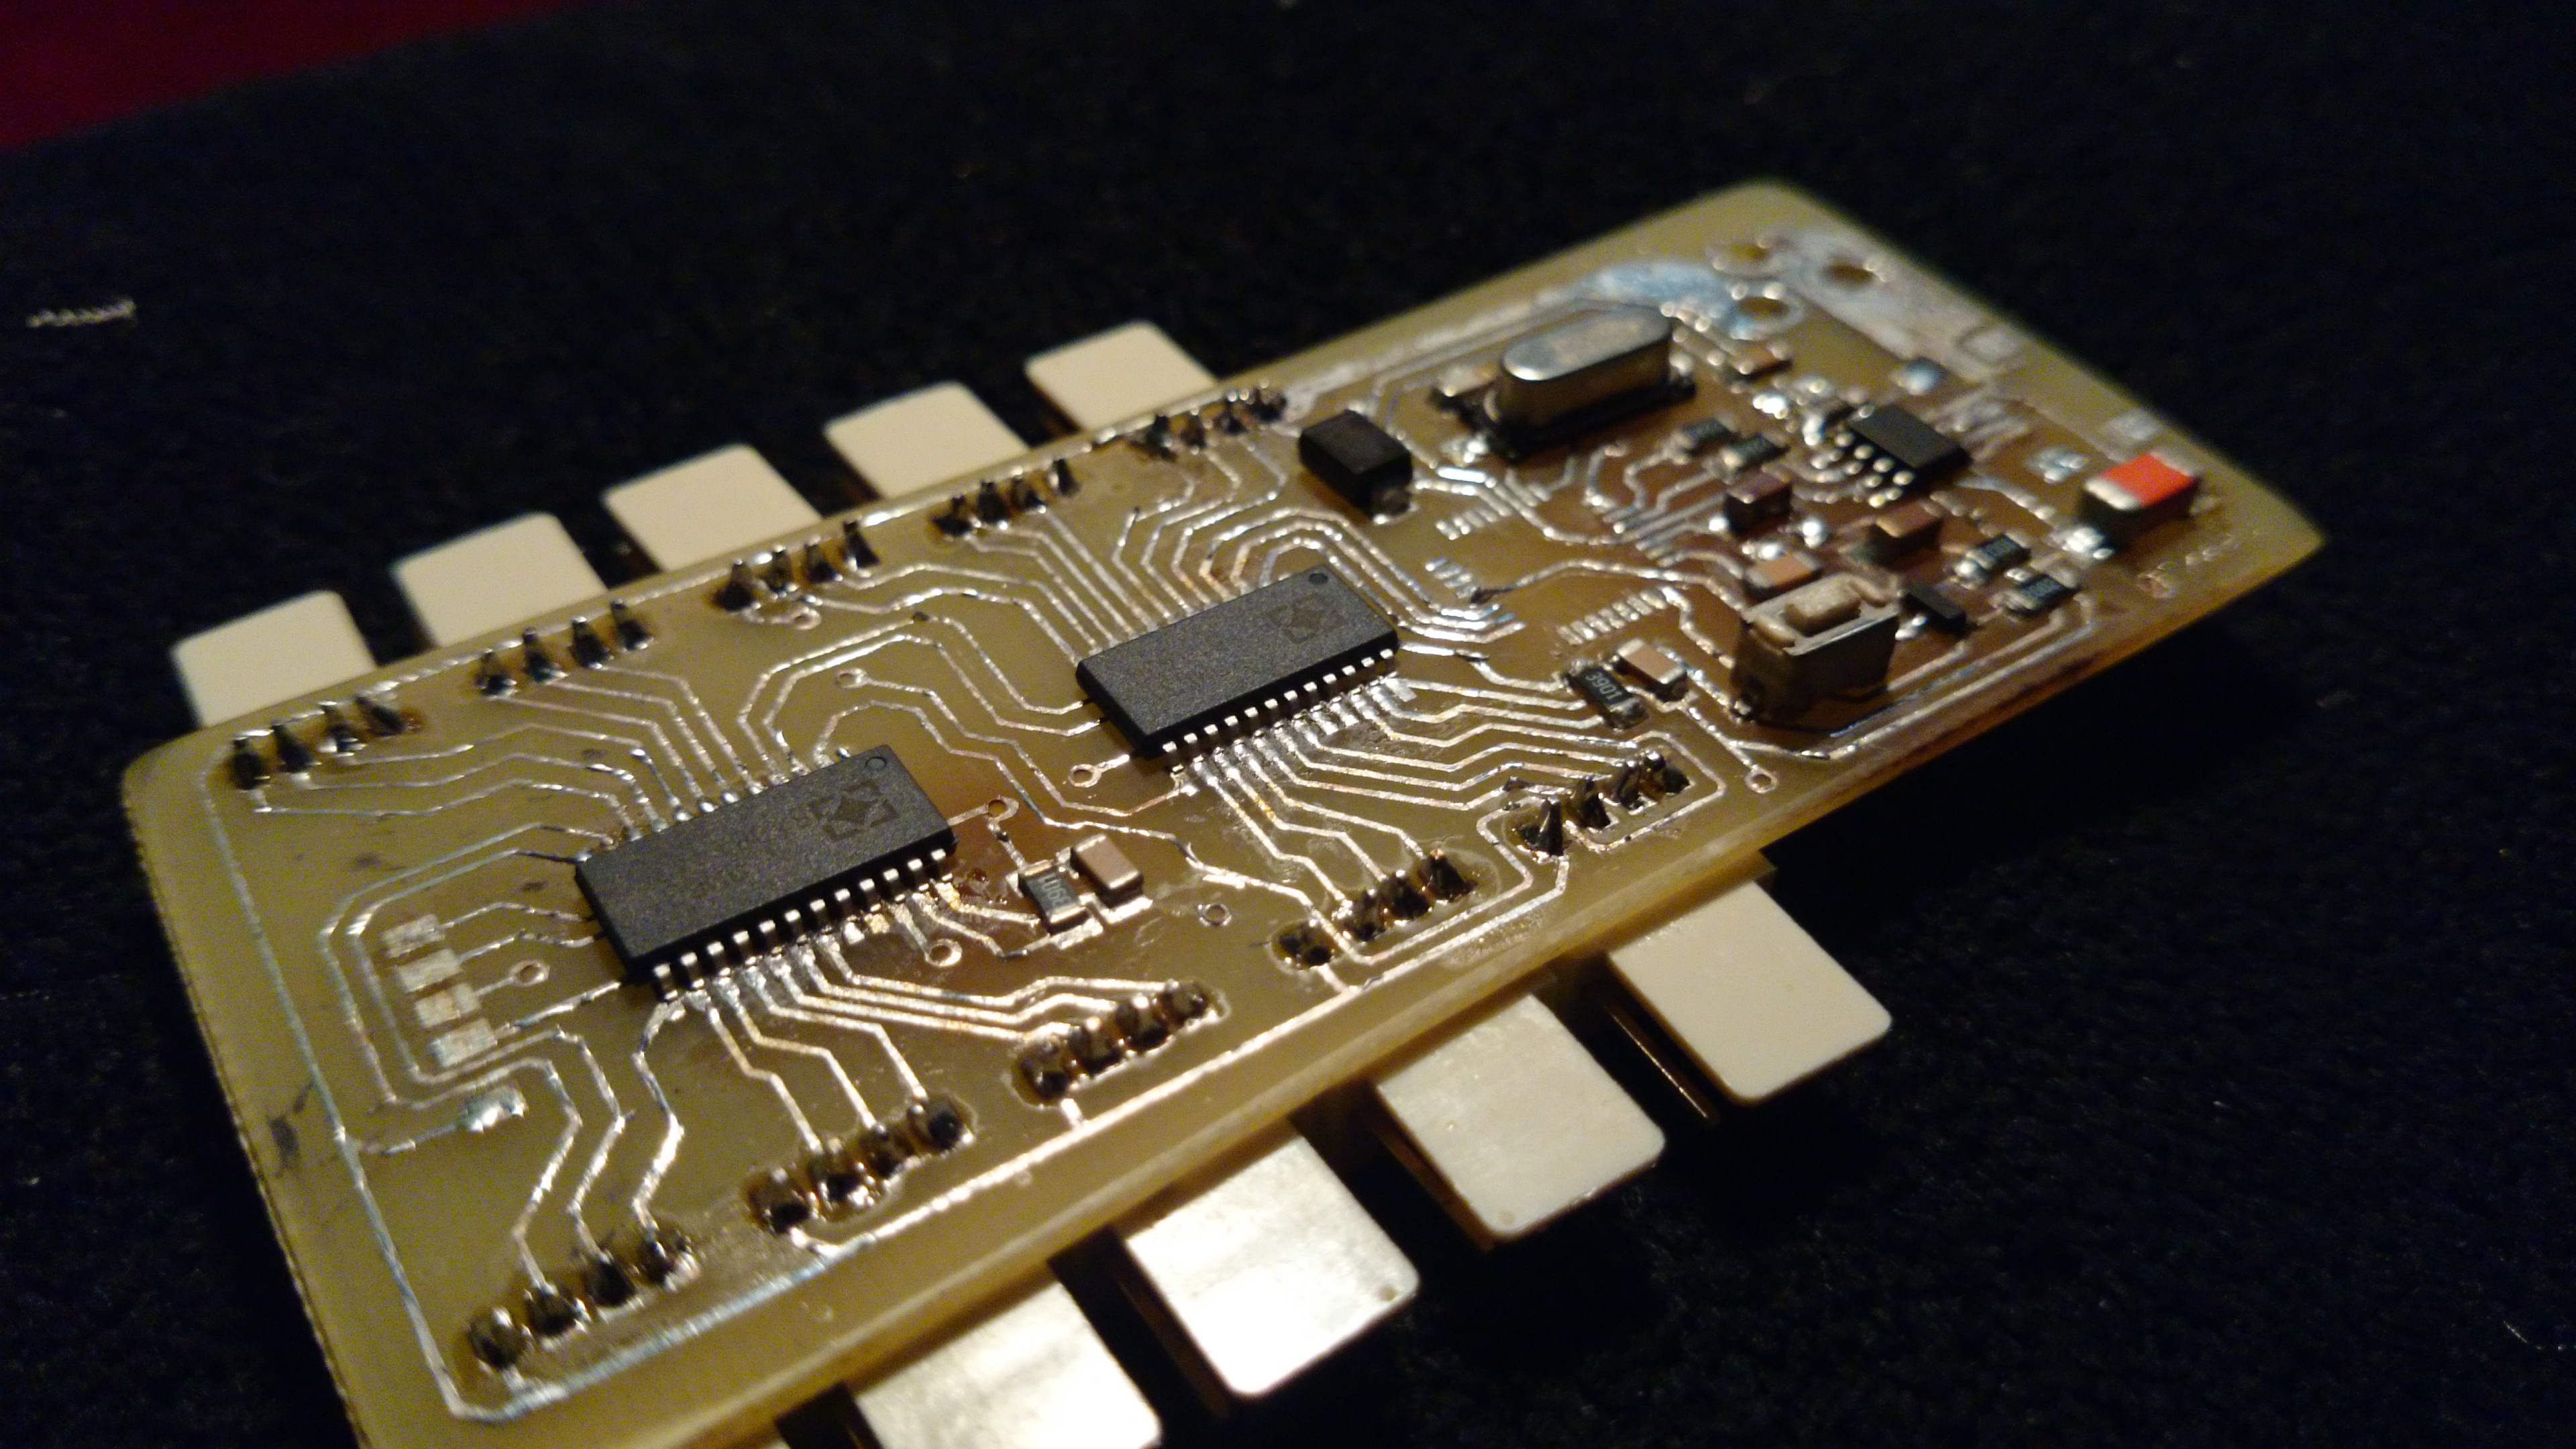
\includegraphics[width = .65\textwidth]{Tesis/Imagenes/prototipo.jpg}
 		\captionof{figure}{Tarjeta de Circuito Impreso finalizada}
	\label{prototipo}
    \end{center} 
\end{figure}


\section{ Comparación con sistemas existentes }

\textit{Utilizando los resultados obtenidos en el capitulo VI (Análisis) es ahora posible cotejar la información y ponerlos uno contra otro para hacer una comparación de los sistemas existentes contra el sistema generado.}


\section{ Análisis costo-beneficio }

\textit{Es necesario justificar la relación costo beneficio del proyecto}

\section{ Trabajo futuro }

\textit{En esta sección caben todas aquellas ideas o mejoras que en algún momento a lo largo del proyecto se pensaron implementar pero no se contemplaron en los objetivos principales o que no tuvieron cabida dentro del lapso de tiempo en el que se desarrolla el proyecto.} 


\section{ Conclusiones }

\textit{Como se observa, desarrollar y redactar un Proyecto y un documento de Tesis, no es una actividad fácil.}

\textit{Conlleva una voluntad férrea, así cómo: una filosofía, mentalidad y aplicación sistémica y sistemática de los conocimientos adquiridos a lo largo de los cursos y del mismo desarrollo del proyecto que, en ocasiones, no sólo es la cúspide de los estudios, sino su reafirmación y mayor integración} \cite{Leopoldo}.




%Capitulo V Conclusión/Valoración de objetivos

\printbibliography[heading=bibintoc,title={BIBLIOGRAFÍA Y WEBGRAFÍA}]
\addappheadtotoc 
\appendixpage 
\appendix  
% APÉNDICE

% En el apéndice tienen cabida todos los documentos que pueden llegar a interrumpir el flujo de lectura en el lector, códigos de programación, hojas de datos, esquemáticos, fotografías, listas de materiales, pruebas realizadas, hojas de datos, no tienen cabida en el cuerpo de la tesis, sin embargo si tienen cabida en el apéndice


\chapter{ Lista de Materiales }

\begin{table}[H]
  \centering
  \begin{tabular}{ c c c c c c }
    \hline\hline
    Cantidad & Componente & No. de Parte&  Costo (USD)\\
    \hline

1 & Raspberry Pi + Accesorios & &$45.00$ \\
1 & Maquilación PCB & OSH Park&  $40.00$ \\
3 & Transductor sensor de corriente alterna &sct-013-000&  $16.20$ \\
1 & Adaptador CA/CA 127v/9v &38K5386 &$20.00$ \\
3 & Modulo RF  &RFM69CW& $17.50$ \\
1 & TQFP-32 Atmega 328p  & 68T2934 &$3.35$ \\
1 & Cristal oscilador 12Mhz & 18C1481 &$1.20$ \\
6 & 0603 Capacitor X7R 100nF 10\% 25v & 06R4927 &$0.19$ \\
5& 0603 Capacitor Cerámico 0603 X5R 10uF 20\% 6v3 & 30K5476&$0.09$ \\
3& 0603 Capacitor Cerámico 0603 X5R 1uF 20\% 6v3 & 93K5996  &$0.19$ \\
1& SMD Capacitor electrolítico aluminio 47uF 16v & 08X4810 &$0.25$ \\
1& 0603 Bobina, 0.04 Ohm, 3A &08X4810 & $0.08$ \\
1& 0805 Led Rojo 1.85v 20mA & 34C8663 & $0.27$ \\
1& Socket miniatura USB 5pin hembra & 16M3869 &$2.30$ \\
1& SOT23 Regulador de voltaje 250mA LDO & 84R5179 & $0.62$ \\
1& SOT89-3 Regulador de voltaje 3.3V 150mA LDO & 71T9800  &$0.91$ \\
1& SOD323 Diodo 100v 150mA & 35K9699 & $0.12$ \\
1& HC-49US Cristal Oscilador 16Mhz 18pF & 60K8254 & $1.25$ \\
5& SOD-523 Diodo ESD 3.3v & 85W3389 & $3.98$ \\
    \hline
  \end{tabular}
 \caption{Lista de materiales }
\end{table}
\newpage

\chapter{ Apéndice de código }

\textit{Poner o no el código del sistema desarrollado es opción totalmente del autor, puede llegar a ocupar demasiadas paginas o prestarse para plagio el colocar el código de programación por lo que es recomendado no colocarlo, ya que no es el medio adecuado para colocarlo, sin embargo puede anexarse el código en un disco compacto para no alterar la estructura del documento de tesis, una alternativa es solo hacer extractos de código de lo mas relevante de los sistemas desarrollados y dar una pequeña explicación y referenciarlos si es necesario, como en el ejemplo siguiente}

\section{ Algoritmo del microcontrolador }

La potencia real es el promedio de la potencia instantánea, el cálculo es relativamente sencillo, primero se debe calcular la potencia instantánea multiplicando la medición de tensión instantánea con la corriente instantánea. Sumamos este valor de potencia instantánea sobre un número de muestras dado, y dividimos entre ese número de muestras es decir: 

\begin{quote}
\begin{verbatim}
for (n=0; n<muestras; n++){    // Tension_instantanea ADC1
  pot_inst = _volt_inst * Corriente_inst;
  suma_pot_inst += pot_inst;
}
pot_real = suma_pot_inst / muestras;
\end{verbatim}
\end{quote}

\subsection{ Tensi\'{o}n media cuadr\'{a}tica (RMS) } 

La raíz cuadrada media se calcula de la forma en que el nombre sugiere primero se eleva al cuadrado, entonces se calcula la media y, finalmente, la raíz cuadrada de la potencia media cuadrática, a continuación se muestra calculo en lenguaje C

\begin{quote}
\begin{verbatim}
for (n=0; n<muestras; n++){ 	  // Corriente_Instantanea ADC2.
  volt_cuadrado = voltaje_inst * voltaje_inst;
  suma_volt_cuadrad += volt_cuadrado;
}
voltaje_medio_cuadratico = sum_squared_voltage / muestras;
voltajeRMS = sqrt(voltaje_medio_cuadratico);
\end{verbatim}
\end{quote}

\chapter{ Hojas de Datos }
\begin{figure}[H]
	\begin{center}
 		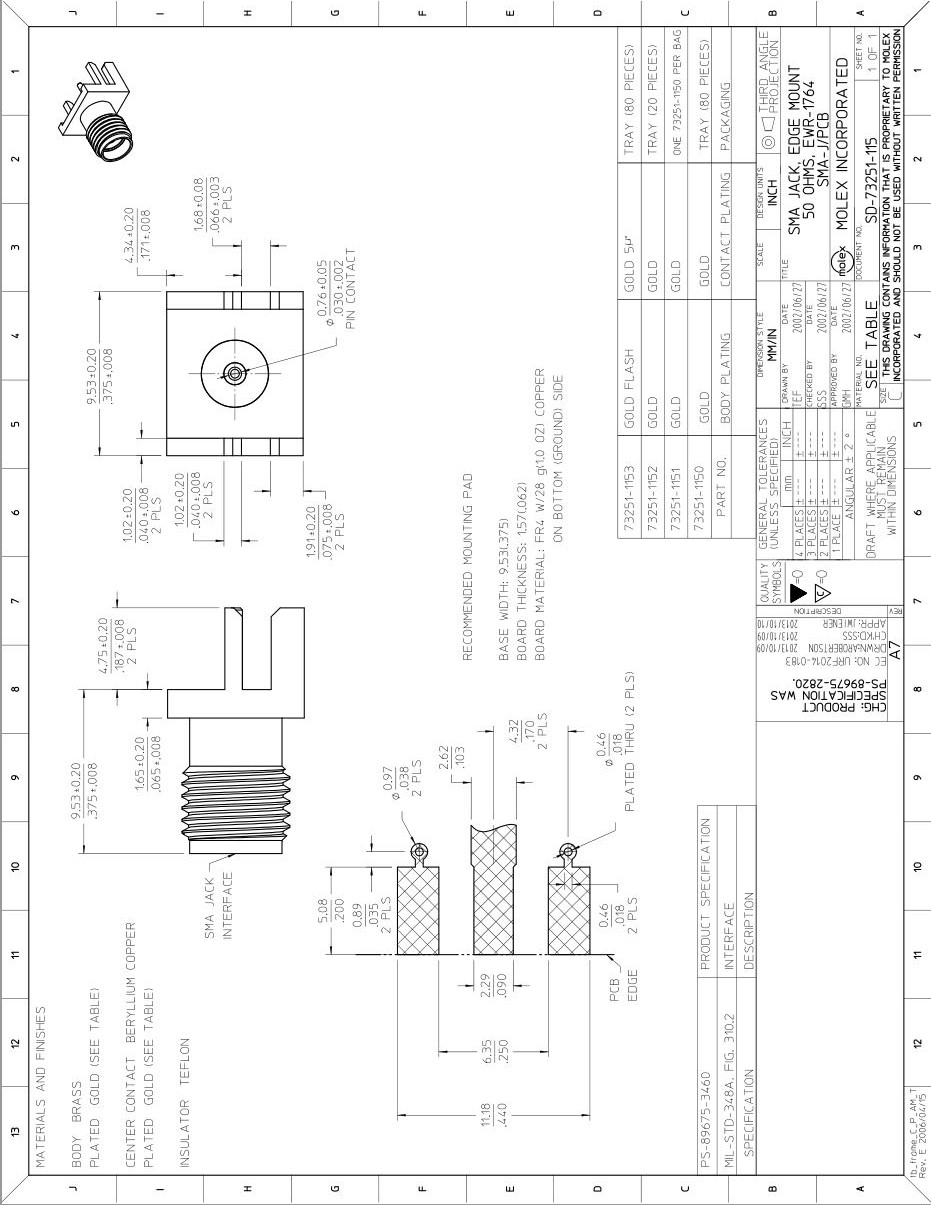
\includegraphics[width = .9\textwidth]{Tesis/Imagenes/Datos.JPG}
 		\captionof{figure}{Hoja de datos del jack SMD para antena de RF} 
	\label{Ap-jackRF}
    \end{center} 
\end{figure}


\end{document}
